%
% IEEE Transactions on Microwave Theory and Techniques example
% Tibault Reveyrand - http://www.microwave.fr
%
% http://www.microwave.fr/LaTeX.html
% ---------------------------------------



% ================================================
% Please HIGHLIGHT the new inputs such like this :
% Text :
%  \hl{comment}
% Aligned Eq. 
% \begin{shaded}
% \end{shaded}
% ================================================



\documentclass[journal]{IEEEtran}

%\usepackage[retainorgcmds]{IEEEtrantools}
%\usepackage{bibentry}  
\usepackage{xcolor,soul,framed} %,caption

\colorlet{shadecolor}{yellow}
% \usepackage{color,soul}
\usepackage[pdftex]{graphicx}
\graphicspath{{../pdf/}{../jpeg/}}
\DeclareGraphicsExtensions{.pdf,.jpeg,.png}

\usepackage[cmex10]{amsmath}
%Mathabx do not work on ScribTex => Removed
%\usepackage{mathabx}
\usepackage{array}
\usepackage{mdwmath}
\usepackage{mdwtab}
\usepackage{eqparbox}
\usepackage{url}
\usepackage{amsmath, amssymb}
\usepackage{graphicx}
\usepackage{hyperref}
\usepackage{cite}
\hyphenation{op-tical net-works semi-conduc-tor}

%\bstctlcite{IEEE:BSTcontrol}


%=== TITLE & AUTHORS ====================================================================
\begin{document}
\bstctlcite{IEEEexample:BSTcontrol}
    \title{Group 8: Online Education Engagement Analysis}
  \author{Andreah Cruz,~\IEEEmembership{Student Member,~IEEE,}
      Bindu Madhavi Edara,~\IEEEmembership{Student Member,~IEEE,}\\
      Harika Eadara,~\IEEEmembership{Student Member,~IEEE,}
      Hemanvitha Katakam,~\IEEEmembership{Student Member,~IEEE,}
      and~Venkata Siddarth Gullipalli\'c,~\IEEEmembership{Student Member,~IEEE}% <-this % stops a space


  }  


% The paper headers
\markboth{IEEE ON ONLINE EDUCATION ENGAGEMENT, DECEMBER~2024
}{Roberg \MakeLowercase{\textit{et al.}}: High-Efficiency Diode and Transistor Rectifiers}


% ====================================================================
\maketitle



% === ABSTRACT ====================================================================
% =================================================================================
\begin{abstract}
%\boldmath
The increasing prevalence of online education, particularly in the post-COVID era, emphasizes the need for enhanced student engagement and personalized learning experiences. This study from the Open University Learning Analytics Dataset (OULAD), captures the demographic, behavioral, and performance data of U.K. students from 2013 to 2014 across multiple virtual learning environments (VLEs). The primary objectives are to analyze engagement patterns, predict student success, evaluate dropout factors, and optimize course design. The dataset’s structure includes student demographics, course assessments, and VLE interactions. This provides a robust foundation for exploratory analysis and modeling which will help us build our data pipeline. Using tools like Power BI, Matplotlib, and Seaborn, we will identify critical factors impacting student performance and engagement. Our methodology includes comprehensive data cleaning, transformation and loading of the data into a staging area, followed by further transformation before it is processed and visualized for analysis. The findings aim to inform personalized learning strategies, enhance course materials, and reduce dropout rates, contributing to a more effective online education environment.
\end{abstract}








% For peer review papers, you can put extra information on the cover
% page as needed:
% \ifCLASSOPTIONpeerreview
% \begin{center} \bfseries EDICS Category: 3-BBND \end{center}
% \fi
%
% For peerreview papers, this IEEEtran command inserts a page break and
% creates the second title. It will be ignored for other modes.
\IEEEpeerreviewmaketitle


% ====================================================================
% ====================================================================
% ====================================================================











% === I. INTRODUCTION =============================================================
% =================================================================================
\section*{Introduction}

The shift toward online education has accelerated significantly in recent years, driven largely by the COVID-19 pandemic and the increasing demand for flexible learning opportunities \cite{Dhawan2020, OECD2020}. While this transition has opened new avenues for education, it has also introduced challenges, particularly in maintaining student engagement, ensuring personalized learning experiences, and reducing dropout rates \cite{Kuh2007, Tinto2012}. These issues show the need for data-driven strategies to optimize online education environments \cite{Siemens2013}.

The Open University Learning Analytics Dataset (OULAD) is a useful resource for understanding these dynamics \cite{Kuzilek2017}. Capturing data from U.K. students between 2013 and 2014, the dataset provides a comprehensive view of student demographics, behavioral interactions within virtual learning environments (VLEs), and academic performance. By leveraging this dataset, we can explore critical factors that influence student engagement, predict success or risk of dropout, and assess the effectiveness of course design.

\subsection*{Motivation}

The increasing reliance on online education in the post-COVID era has highlighted significant disparities in student engagement and academic outcomes. Despite its accessibility and flexibility, online learning often lacks the immediacy of traditional classroom interactions, leading to challenges in sustaining student motivation, fostering active participation, and preventing dropout. These challenges are particularly pronounced among students from diverse demographic and socioeconomic backgrounds, as they encounter unique barriers to success in virtual environments \cite{Kuzilek2017}.

Addressing these challenges requires us to use data-driven insights to understand and optimize the online learning experience. The Open University Learning Analytics Dataset (OULAD) provides this opportunity to analyze the interaction between student behavior, demographic factors, and academic performance. By identifying the factors that drive or hinder success in online education, we may be able to contribute to the knowledge of how to create equitable and effective learning environments.  Our deeper understanding of these dynamics can inform interventions that improve student outcomes and foster a more inclusive educational landscape.

\subsection*{Problem Definition}

Despite the potential of online education, student retention and success remain significant challenges. High dropout rates, low engagement, and inequities in learning outcomes persist across virtual learning environments (VLEs). Furthermore, current educational technologies often fail to adapt to individual learning needs, resulting in a one-size-fits-all approach that may alienate or under-serve certain students.

\subsection*{Objectives}

Our goal is to analyze student engagement patterns, evaluate demographic and socioeconomic influences on performance, and identify key factors contributing to dropout rates. Through these analyses, we seek to uncover actionable insights for enhancing online education.

\subsection*{Expected Outcomes}

Ultimately, the findings from this study are expected to inform personalized learning strategies, improve course materials, and contribute to a more inclusive and effective online education system. By addressing the core challenges in online learning, this project intends to advance the field of education and support students in achieving their academic goals.




% === II. Harmonically-Terminated Power Rectifier Analysis ========================
% =================================================================================
\section{Methodology}

In order to understand our data, certain steps must be achieved to implement the final part of the visualization. Our approach involves preprocessing the dataset—cleaning missing values, handling outliers, and transforming features—to ensure data integrity and usability. Visualization and statistical tools, such as Power BI, Matplotlib, and Seaborn, will support our efforts in identifying meaningful trends and patterns \cite{Hunter2007, Waskom2021}.

% =======
% FIG. 01
% =======
\begin{figure}
  \begin{center}
  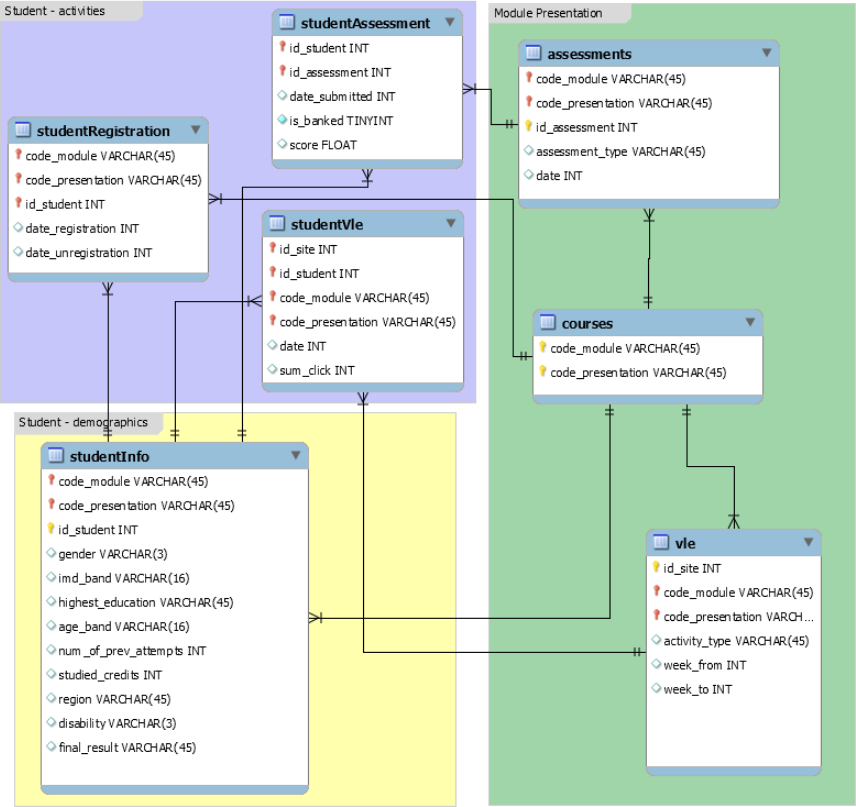
\includegraphics[width=3.5in]{photo/schema.PNG}\\
  \caption{Illustration the Entity-Relationship structure of the Open University Learning Analytics Dataset (OULAD)}
  \label{pu_image}
  \end{center}
\end{figure}


\subsection*{Business Understanding}

We seek to analyze and optimize student engagement and performance in online education environments by leveraging insights from the Open University Learning Analytics Dataset (OULAD). The objective is to identify factors that influence learning outcomes, predict at-risk students, and evaluate the effectiveness of course materials. By understanding these dynamics, institutions can make informed decisions to enhance student retention and success rates. 

To achieve this, the team explored existing literature and practices in learning analytics to determine effective approaches for analyzing demographic, behavioral, and academic data. Using insights from these studies, a structured plan was developed to preprocess and analyze the dataset, integrating data cleaning, visualization, and modeling techniques. This systematic approach ensures transparency and accuracy in identifying actionable strategies for improving online education outcomes.


\subsection*{Data Understanding}
The Open University Learning Analytics Dataset (OULAD) was carefully probed to understand its structure and content. This publicly available dataset provides detailed insights into student interactions, demographics, and academic outcomes across various courses offered by the Open University. It consists of multiple interconnected tables, each containing specific information such as student registration details, demographic data, virtual learning environment (VLE) interactions, assessment records, and course outcomes.

Key features of the dataset include student engagement metrics (e.g., click counts on VLE activities), demographic attributes like age, gender, and educational background, and academic results such as pass, fail, or withdrawal status. The data is organized in a relational structure, making it possible to analyze the connections between students' activities, demographics, and academic performance.

To gain a deeper understanding, initial visualizations and analyses were performed using tools like Tableau, Power BI, and Python libraries such as Matplotlib and Seaborn. This helped identify trends and anomalies, such as missing values or outliers, and highlighted potential relationships between different attributes. These insights formed the basis for preparing the data for further analysis, ensuring its quality and relevance for the study.

\subsection*{Data Preparation}
During the data preparation process, several anomalies were identified and addressed. Columns with a high percentage of missing values (e.g., over 80\%)—particularly those related to dates—were dropped, as the missing data was too extensive to reliably impute. Additionally, columns deemed unnecessary for visualization or analysis were removed to streamline the dataset. For columns with a smaller proportion of missing values (5\% or less), appropriate methods were applied to fill in the gaps.

To simplify visualization and enhance interpretability, redundant columns were removed and replaced with consolidated information. For example, the dataset originally included 13 regions, which made pattern recognition in visualizations more challenging. These regions were grouped into six broader categories to improve clarity. Outliers were also addressed, with extreme values either removed or capped based on logical thresholds to maintain data integrity. Throughout the process, preserving the integrity and usability of the data was prioritized to ensure that the dataset remained accurate and meaningful for further analysis.

\subsection*{Data Modeling}
The data model for this project was designed to integrate, process, and analyze student engagement data within the Virtual Learning Environment (VLE) effectively. It organizes key components, such as student demographics, module information, assessments, and interaction data, into a relational structure. This structure effectively supports our data exploration, visualization, and the generation of actionable insights.


\subsection*{Model Evaluation}
Evaluations serve as critical metrics to assess the performance and impact of data visualizations or dashboards. These metrics focus on understanding how effectively the visualization communicates information and supports decision-making processes. Key performance metrics include clarity, engagement, accuracy, and efficiency. Clarity refers to the ease with which the audience can comprehend the presented information, while engagement evaluates the ability of the visualization to capture and maintain user attention. Accuracy ensures that the data is represented without misinterpretation, and efficiency measures the time required for users to derive actionable insights.

Additionally, impact metrics assess how the visualization contributes to practical outcomes. User feedback, interaction data, and time-to-insight are commonly used methods to evaluate performance. In this case the team performed the evaluations ourselves. 

Effective visualizations facilitate better decisions by presenting actionable insights, which can be evaluated by comparing outcomes before and after implementation. These metrics collectively ensure that the visualization not only meets technical standards but also delivers meaningful value to its intended audience.

\subsection*{Model Deployment}
To deploy our model, we will utilize Power BI to create an interactive and comprehensive dashboard after completing the primary data preparation in Jupyter Notebooks. While Jupyter Notebooks is effective for initial data exploration and visualization, Power BI offers a more extensive range of visualization options and is better suited for our target audience. Additionally, Power BI allows for the application of simplistic filters and further data preparation directly within the platform, enabling users to refine and customize the data as needed for deeper insights and enhanced user experience. This flexibility ensures that our dashboard is both functional and audience-friendly.

\section{Data Flow and Preparation}

\subsection*{Data Exploration}
In the data exploration phase of our project, we conducted a comprehensive analysis of the Open University Learning Analytics Dataset (OULAD) to gain deep insights into its structure, dimensions, and key variables pertinent to student engagement and performance. Utilizing visualization techniques such as histograms and heatmaps with tools like Matplotlib and Seaborn, we uncovered patterns and distributions within the data as depicted in Figure~\ref{distribution} These visualizations helped us identify correlations between student demographics, virtual learning environment (VLE) interactions, and academic outcomes.

% =======
% FIG. 02
% =======
\begin{figure}
  \begin{center}
  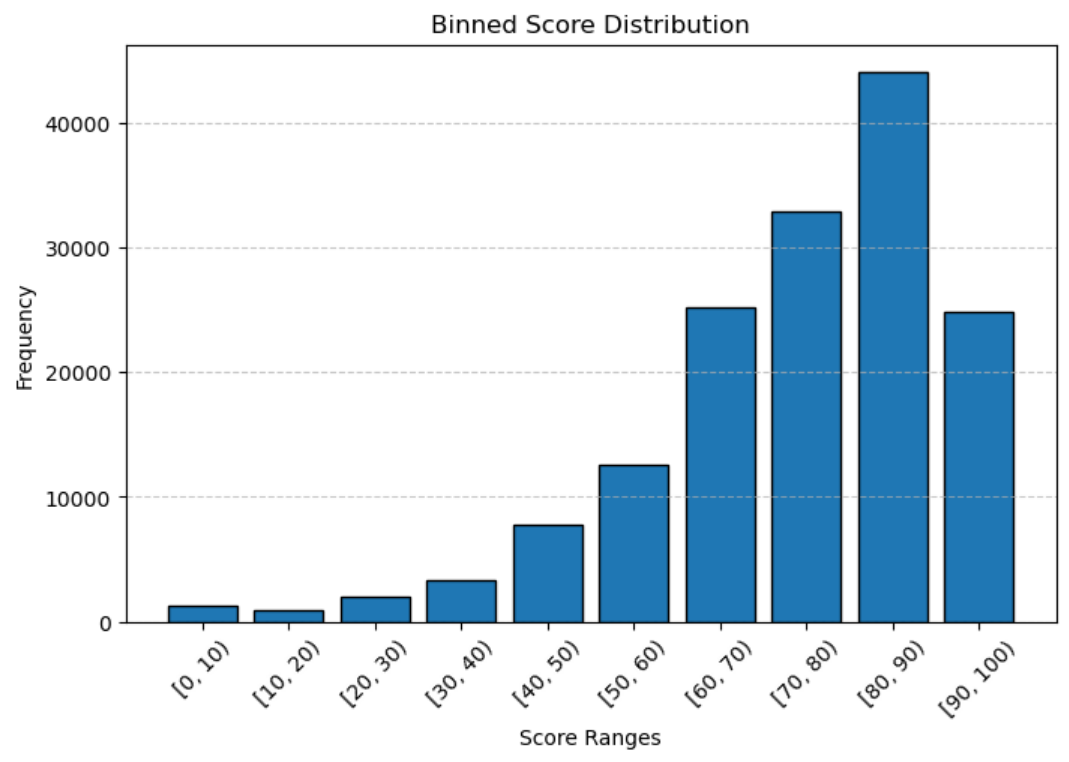
\includegraphics[width=3.5in]{photo/distrib.PNG}\\
  \caption{Score distribution diagram}
  \label{distribution}
  \end{center}
\end{figure}

\begin{figure}
  \begin{center}
  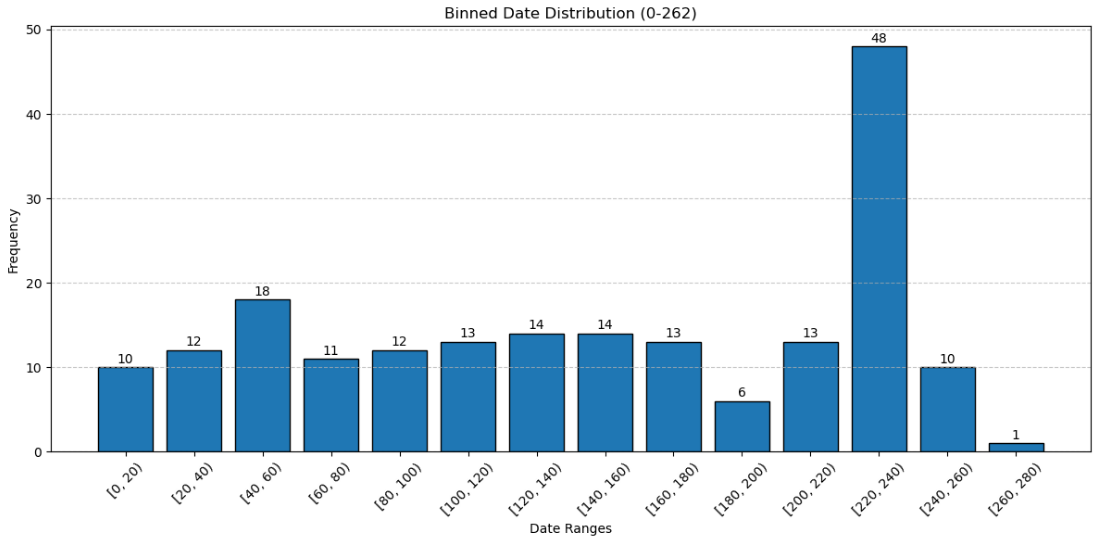
\includegraphics[width=3.5in]{photo/uniformdate.PNG}\\
  \caption{Date distribution diagram}
  \label{unidate}
  \end{center}
\end{figure}

Simultaneously, we thoroughly assessed data quality by identifying and addressing anomalies. We carefully looked at null values, outliers, and duplicate records, recognizing that these could significantly impact our analyses. Missing data in critical variables like assessment scores and VLE activities were carefully examined to determine their implications. Outliers were investigated to understand whether they represented data entry errors or genuine extreme cases. Duplicate records were removed to maintain data integrity.


\subsection*{Dataset Description}

A total of eight files were generated as part of our data collection process. These files include: 

\begin{itemize}
    \item \textbf{anoymisedData:} This file contains anonymized information about assessments conducted within each module presentation. Although it was provided it wasn't used as the file contained too many null values (as its anonymised). It was dropped as it did not provide much for the findings we are going for. 
    
    \item \textbf{courses:} This file contains information about the modules and their presentations, including the module code (\texttt{code\_module}), presentation code (\texttt{code\_presentation}), and the length of the presentation in days (\texttt{length}). It provides an overview of the structure and schedule of courses offered by the Open University.

    \item \textbf{assessments:} This file details the assessments associated with each module presentation, such as the assessment type (\texttt{assessment\_type}), final submission date (\texttt{date}), and weight (\texttt{weight}) as a percentage of the overall grade. It helps analyze the role of different assessments in student performance.

    \item \textbf{vle:} This file captures information about the materials available on the Virtual Learning Environment (VLE), including the type of activity (\texttt{activity\_type}) and the weeks when the materials are accessible (\texttt{week\_from} and \texttt{week\_to}). This data is useful for understanding resource availability and its correlation with student engagement.

    \item \textbf{studentInfo:} This dataset provides demographic details and academic outcomes for students, such as gender (\texttt{gender}), age band (\texttt{age\_band}), highest education level (\texttt{highest\_education}), region (\texttt{region}), and final result (\texttt{final\_result}). It offers insights into how personal characteristics influence learning outcomes.

    \item \textbf{studentRegistration:} This file includes data on student registration and unregistration, with attributes like registration date (\texttt{date\_registration}) and unregistration date (\texttt{date\_unregistration}). It helps identify patterns of enrollment and withdrawal.

    \item \textbf{studentAssessment:} This dataset logs individual student assessment scores (\texttt{score}), submission dates (\texttt{date\_submitted}), and whether the assessment result was carried over from a previous presentation (\texttt{is\_banked}). It supports the analysis of assessment performance and submission behavior.

    \item \textbf{studentVle:} This file records student interactions with VLE materials, including the number of clicks (\texttt{sum\_click}) and the date of interaction (\texttt{date}). It is key to understanding engagement with online learning resources.

\end{itemize}

\subsection*{Data Preparation and Cleaning}

The data preparation and cleaning phase of our project was critical. In total, eight datasets were collected for analysis. Out of these, the \texttt{studentVLE} and \texttt{courses} files were clean, containing no missing data. However, some files, such as \texttt{anonymisedData}, \texttt{studentRegistration}, and \texttt{vle}, had over 80\% missing data. This amount of missing data was deemed too excessive to handle effectively, leading us to drop these columns entirely. Attempting to use imputation methods on such sparse data would have distorted the distribution, resulting in inaccurate analyses and misleading outcomes.

For datasets with less than 5\% missing data, we implemented appropriate replacement methods tailored to each column's distribution. This ensured the integrity of the dataset while maintaining its usability for further analysis.

\subsection*{Handling Missing Data}
The \texttt{studentAssessment} file, for instance, contained 173 missing values in the \texttt{score} column, accounting for less than 1\% of the dataset. Since the distribution of the \texttt{score} column was left-skewed, median imputation was employed. The median is less influenced by extreme values and better represents the central tendency in skewed distributions. This approach ensured that the dataset's underlying patterns remained intact.

Similarly, in the \texttt{assessments} file, the \texttt{date} column had 11 missing values, constituting 5\% of the column. Since the data distribution was uniform, we used random seeding to fill in the missing values, ensuring that the replacement preserved the original distribution.

% =======
% FIG. 05
% =======
\begin{figure}
  \begin{center}
  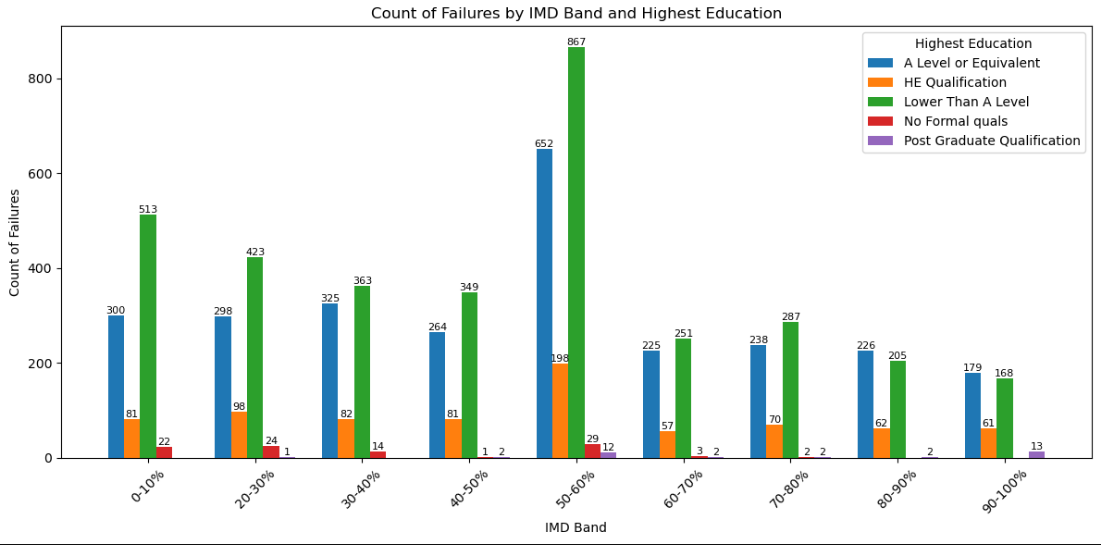
\includegraphics[width=3.5in]{photo/clusteredimd.PNG}\\
  \caption{Misuse of mode imputation of imd\_band resulting in improper distribution}
  \label{clutteredimd}
  \end{center}
\end{figure}

% =======
% FIG. 05
% =======
\begin{figure}
  \begin{center}
  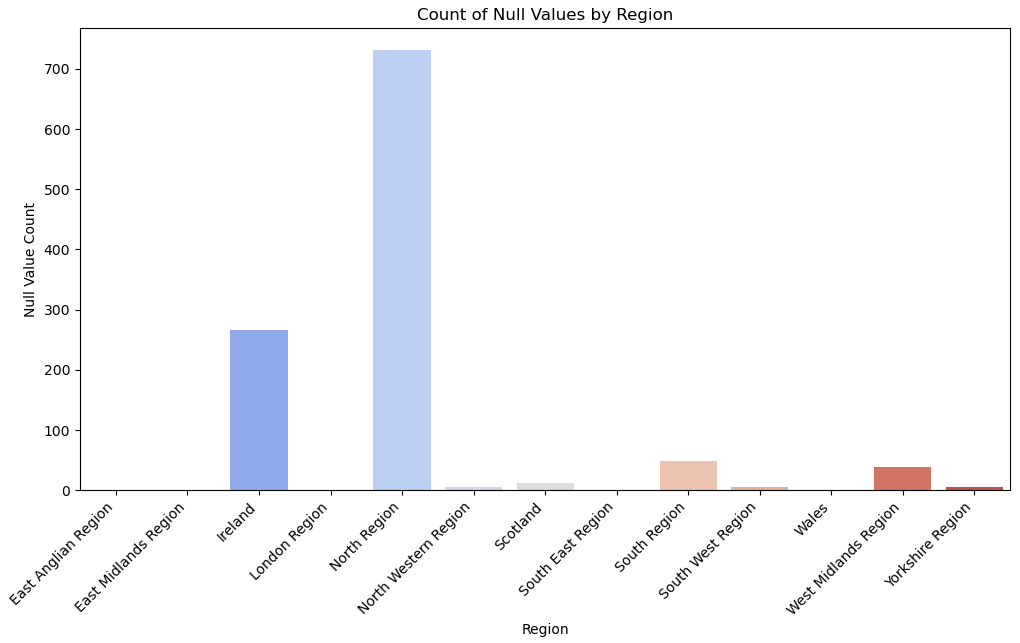
\includegraphics[width=3.5in]{photo/ncr.PNG}\\
  \caption{Count of null values for the region column of the studentInfo file}
  \label{ncr}
  \end{center}
\end{figure}

% =======
% FIG. 05
% =======
\begin{figure}
  \begin{center}
  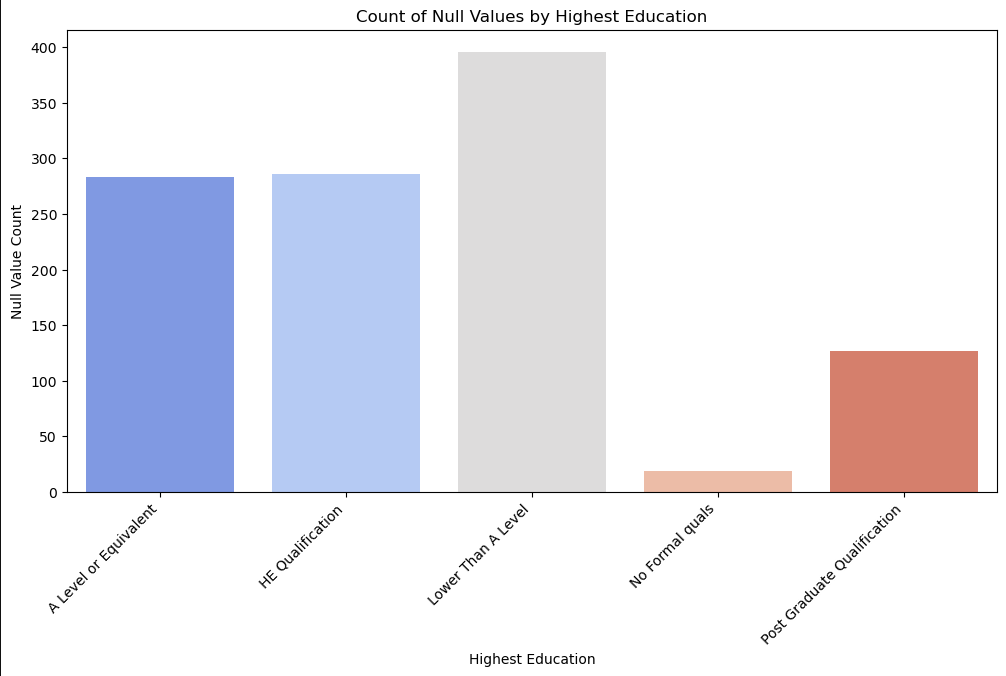
\includegraphics[width=3.5in]{photo/henc.PNG}\\
  \caption{Count of null values for the highest\_education column of the studentInfo file}
  \label{henc}
  \end{center}
\end{figure}

The most challenging case was the \texttt{studentInfo} file, where the \texttt{imdBand} column contained 1,111 missing values, representing 2\% of the column. A straightforward mean, median, or mode imputation would have concentrated all data points in a single bin (the 50\%–60\% band), oversimplifying the distribution and failing to account for contextual factors, as depicted in Figure~\ref{clutteredimd}. Upon closer inspection, we found that most of the missing values were associated with students from the North Region with a highest education level of \textit{Lower Than A Level} as shown in Figure~\ref{ncr} and Figure~\ref{henc}. To address this, we split the data into two subsets: one for this specific group and another for the remaining data. Mode imputation was applied separately to these subsets, as it is more appropriate for categorical variables. For students in the North Region with \textit{Lower Than A Level}, we replaced missing values with the mode of that subset, while for the rest of the data, the overall mode was used. This approach allowed us to preserve the distribution and maintain the dataset's integrity.

\subsection*{Outlier Detection and Treatment}

While some files had no missing data, they contained outliers that needed to be addressed. The \texttt{studentVLE} file, in particular, presented significant challenges with outliers in the distribution of student clicks on VLE materials across module presentations. During our midterm presentation, we initially used median replacement to handle outliers due to its simplicity. However, upon further investigation, we realized this approach compromised the integrity of the dataset, as it artificially set the second quartile (median) to 2.5 for every module presentation. Extreme cases, such as students recording 4,000 or even 7,000 clicks, were outliers that required more careful handling, as depicted in Figure~\ref{fig:barplotcleaned}.

\begin{figure}[h]
    \centering
    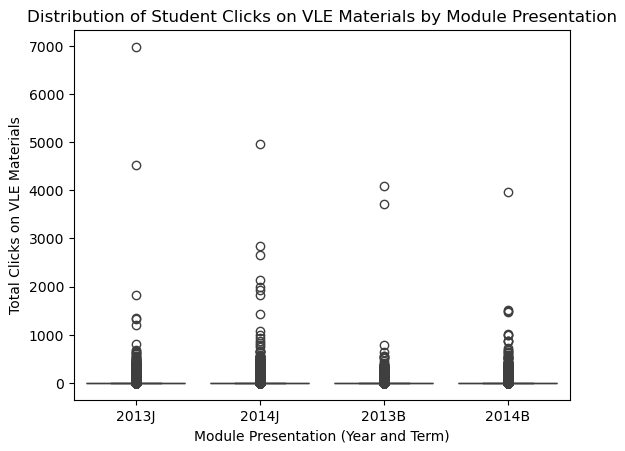
\includegraphics[width=\linewidth]{photo/barplot.PNG}
    \caption{Distribution of Student Clicks on VLE Materials After Cleaning Outliers}
    \label{barplot}
\end{figure}


To resolve this, we decided to drop duplicates. Rather than removing duplicates based on columns like \texttt{id\_student}, \texttt{id\_site}, or \texttt{date}, we focused on ensuring that each record represented unique student clicks for each module. Additionally, we capped the data at 2,000 clicks, as values beyond this threshold were deemed unrealistic and contributed little to the analysis. This approach preserved the data's meaningful patterns while reducing the influence of extreme values.

\begin{figure}[h]
    \centering
    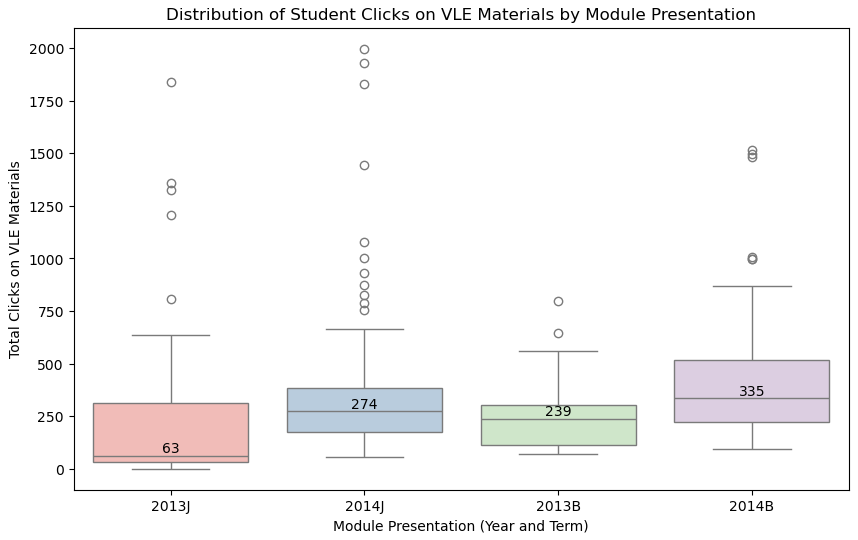
\includegraphics[width=\linewidth]{photo/barplotcleaned.PNG}
    \caption{Distribution of Student Clicks on VLE Materials After Cleaning Outliers}
    \label{fig:barplotcleaned}
\end{figure}

\subsection*{Region Simplification}
Finally, we simplified the region information in the \texttt{studentAssessment} file. Initially, the dataset included 13 regions, which created unnecessary clutter and made visualizations less effective as shown in Figure~\ref{clutteredb}. To enhance interpretability and streamline the analysis, we grouped the regions into broader categories: London, Scotland, Wales, and Ireland. However since the rest of the regions (ie. East Anglian Region, East Midlands Region, North Region, North Western Region, South East Region, South Region, South West Region, West Midlands Region, and Yorkshire Region) were from London our team decided it was best to divide it by the affluence of the region as shown in Figure~\ref{sixregbg}\cite{IMD2019}. This aggregation made the dataset more manageable and provided clearer insights during visualization and analysis.

% =======
% FIG. 04
% =======
\begin{figure}[h]
    \centering
    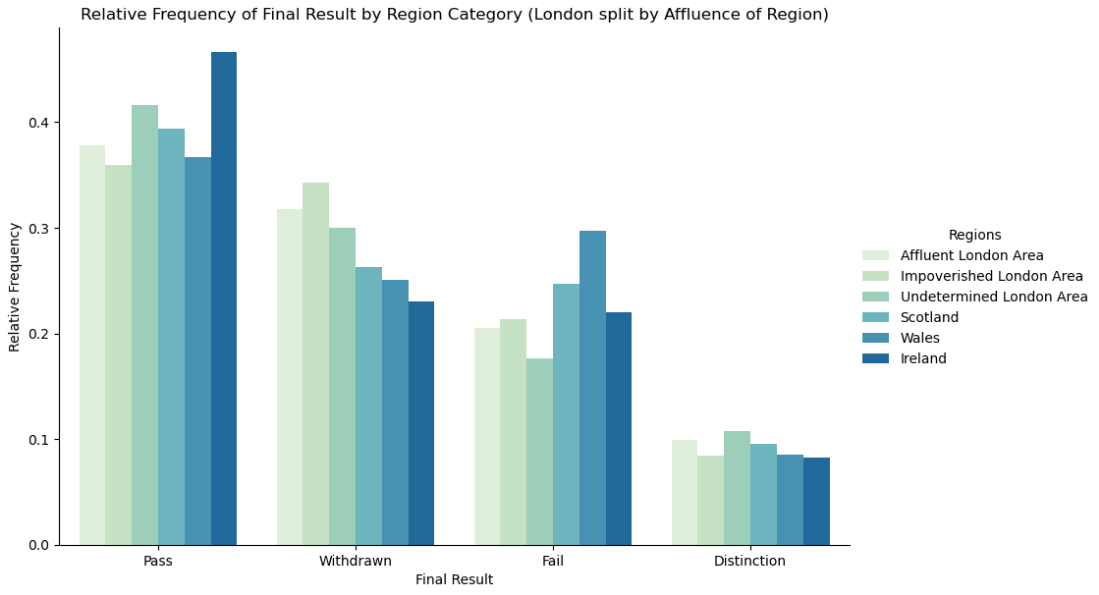
\includegraphics[width=0.40\textwidth]{photo/sixregionbg.PNG}
    \caption{Clustered bar chart before regions were simplified}
    \label{sixregbg}
\end{figure}

\begin{figure}[h]
    \centering
    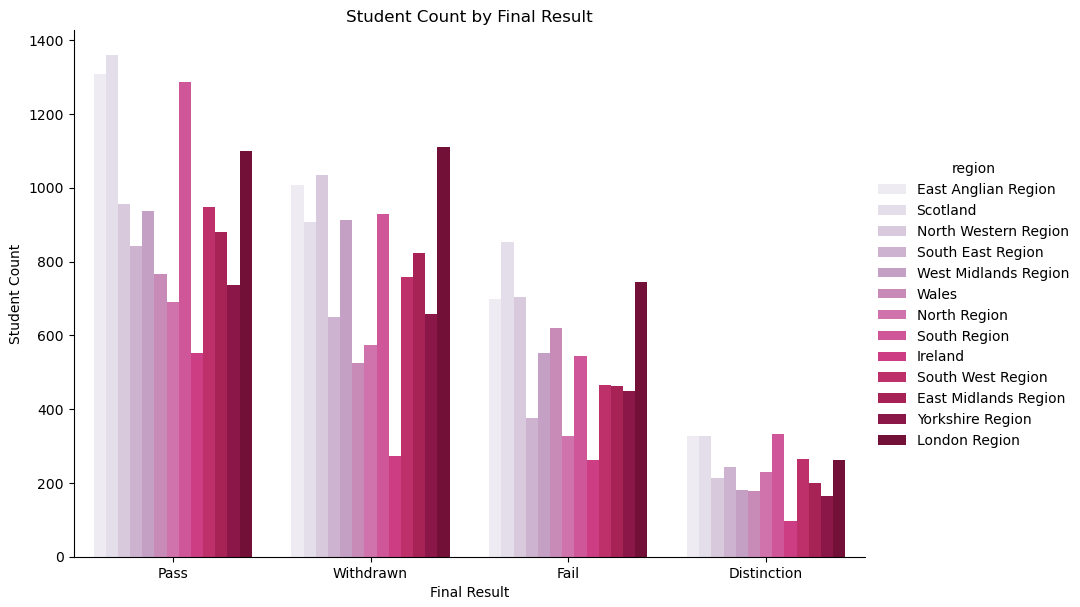
\includegraphics[width=0.40\textwidth]{photo/clutteredbar.PNG}
    \caption{Clustered bar chart after regions were simplified}
    \label{clutteredb}
\end{figure}

% =======
% FIG. 04
% =======

By addressing missing data, outliers, and redundant information through these targeted strategies, we ensured the dataset's quality and integrity.

\subsection*{Data Preparation Using Power BI}

After completing data cleaning and preprocessing in Python, we proceeded with data preparation in Power BI to enhance our visualizations. Our team extensively utilized Power BI tools such as \textit{Measure}, \textit{New Column}, and \textit{New Table} to create additional variables and datasets required for specific analyses. For example, we transformed the \texttt{final\_result} variable into a binary \texttt{Pass\_Result} column—assigning 1 to \textit{Pass} and \textit{Distinction}, and 0 to \textit{Withdrawn} and \textit{Fail}—which was frequently used in our visualizations.

We also binned the score data similarly to our approach in Python. Utilizing the \textit{New Table} tool allowed us to examine the relationship between \texttt{sum\_clicks} and \texttt{score} more thoroughly to determine if increased interaction correlated with higher scores. Interestingly, we discovered that increased clicks did not necessarily lead to better scores. The \textit{Measure} tool was specifically employed to calculate the average pass rate based on clicks.

\section{Modeling}
A data model serves as the backbone of our analysis, providing the foundation for generating insights that inform recommendations and improve decision-making processes in online education systems.
\subsubsection{Core Data Model Design}
The model incorporates the following components:
\begin{itemize}
    \item \textbf{Student Demographics:} This dimension captures information about students, including gender, age band, region, highest education level, socio-economic status (IMD band), and disabilities. This data links directly to enrollment and engagement records to contextualize individual and group performance trends.
    \item \textbf{Student Enrollment:} Enrollment and registration data track student participation across module presentations, linking demographic attributes to course outcomes. It includes timestamps for registration and withdrawal, providing insights into dropout patterns.
    \item \textbf{Course and Module Information:} The model integrates course codes, module identifiers, and presentation schedules, allowing detailed tracking of learning paths. Modules are linked to assessments and VLE interaction data.
    \item \textbf{Assessments:} Assessment data capture student performance in tutor-marked, computer-marked, and final exam assessments. Attributes such as scores, submission dates, and weights contribute to understanding factors that influence success or failure.
    \item \textbf{VLE Interactions:} Interaction logs track clicks and engagement with course resources, including PDFs, HTML materials, and forum activities. This data is crucial for evaluating student engagement.
    \item \textbf{Outcomes:} The outcomes table consolidates information about pass, fail, or withdrawal statuses, enabling performance evaluation.
\end{itemize}

\subsubsection{Implementation and Tools}
The model follows a \textit{relational schema} (e.g., star schema), as depicted in Figure~\ref{pu_image}, integrating data dimensions with fact tables to ensure scalability and efficiency. \textit{Power BI} was used to implement relationships, clean data, and establish data pipelines better. Figure~\ref{fig:method} highlights the data flow pipeline, detailing steps from collection to visualization. Visualizations (Figure~\ref{fig:relations}) were designed to showcase trends and insights, particularly in demographic influences, engagement levels, and course outcomes.

\subsubsection{Challenges and Scalability}
Developing this model required addressing challenges such as inconsistent data formats, missing values, and normalization issues. The model ensures scalability for large datasets, allowing integration with future modules or enhanced engagement metrics.

This data model serves as the backbone of our analysis, providing the foundation for generating insights that inform recommendations and improve decision-making processes in online education systems.

\begin{figure}[h]
    \centering
    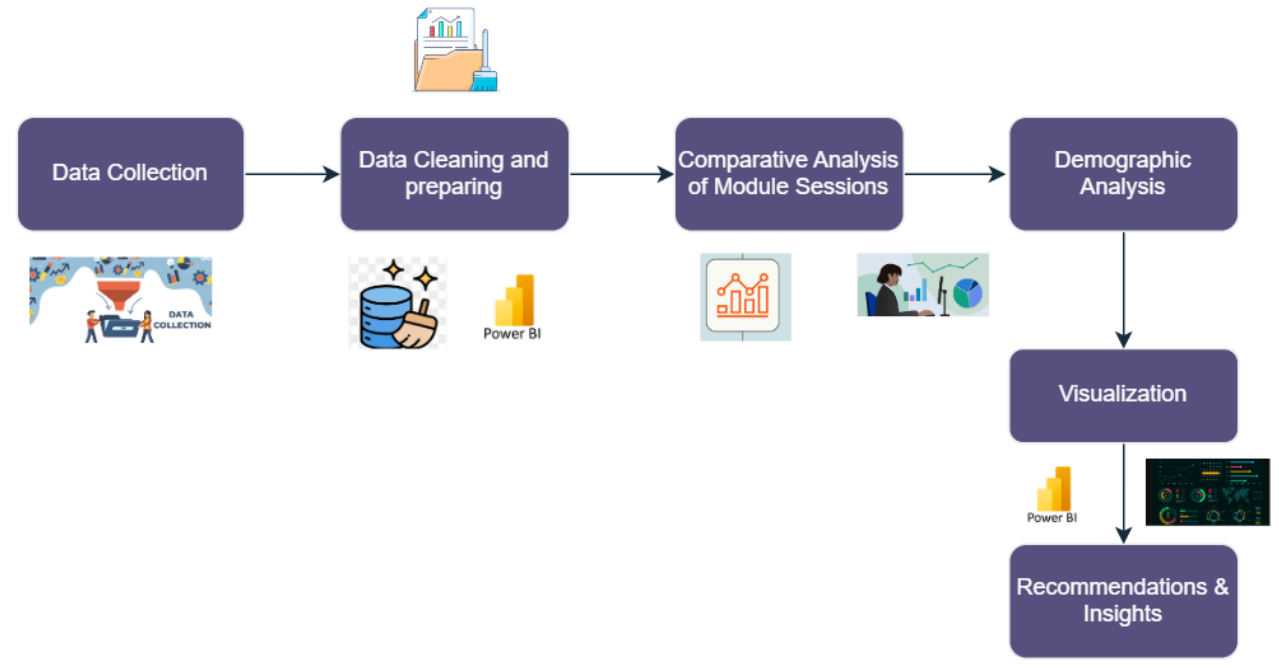
\includegraphics[width=\linewidth]{photo/method.PNG}
    \caption{Data flow pipeline from collection to visualization.}
    \label{fig:method}
\end{figure}

\begin{figure}[h]
    \centering
    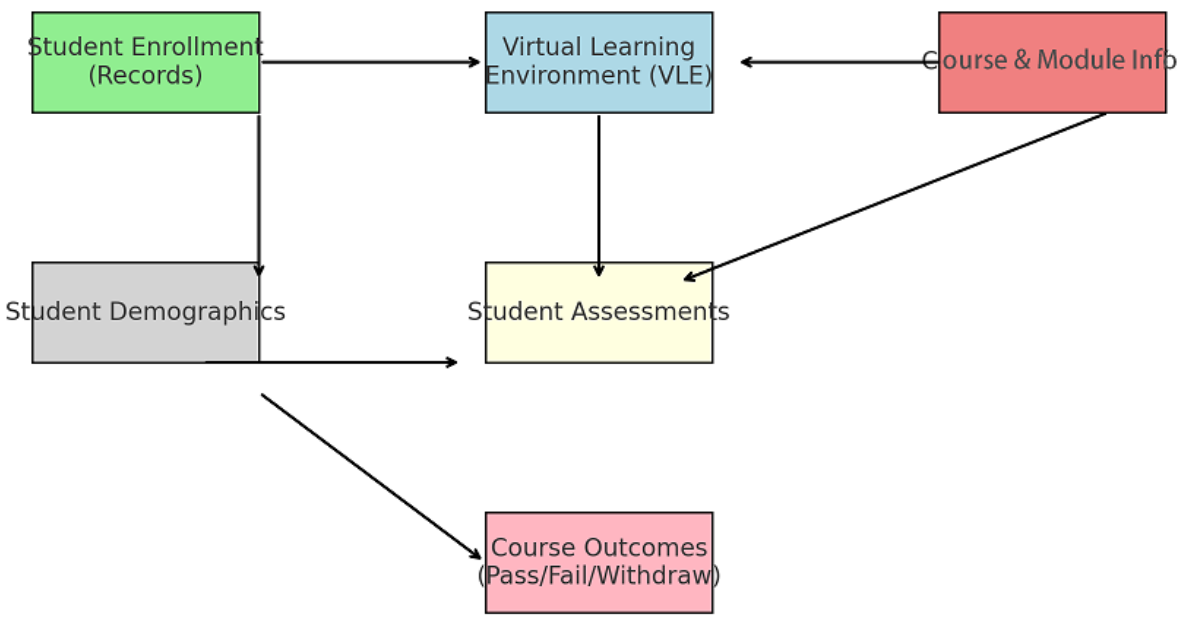
\includegraphics[width=\linewidth]{photo/relations.PNG}
    \caption{Data Pipeline Model for Student Engagement and Course Outcomes.}
    \label{fig:relations}
\end{figure}

\section{Evaluation and Discussion}

The evaluation of our Power BI dashboard focuses on its effectiveness in communicating critical insights and addressing key questions related to student engagement and performance in online education. By thoroughly examining each visualization, we assess its contribution to the overall narrative and its alignment with our project's objectives, ensuring a comprehensive evaluation of results and appropriate reflection on underlying assumptions.

% Insert images
\begin{figure}[h!]
    \centering
    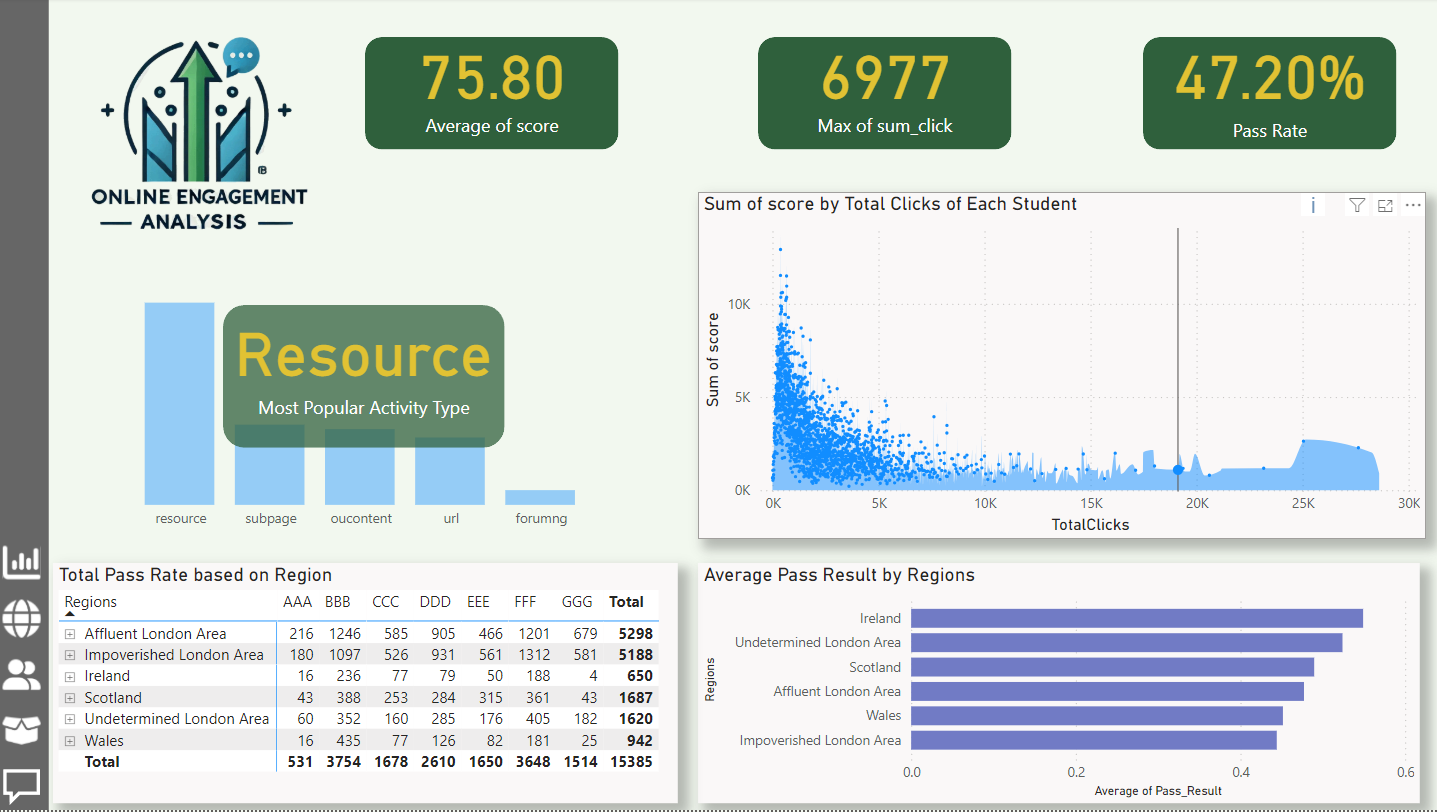
\includegraphics[width=0.45\textwidth]{photo/d1.PNG}
    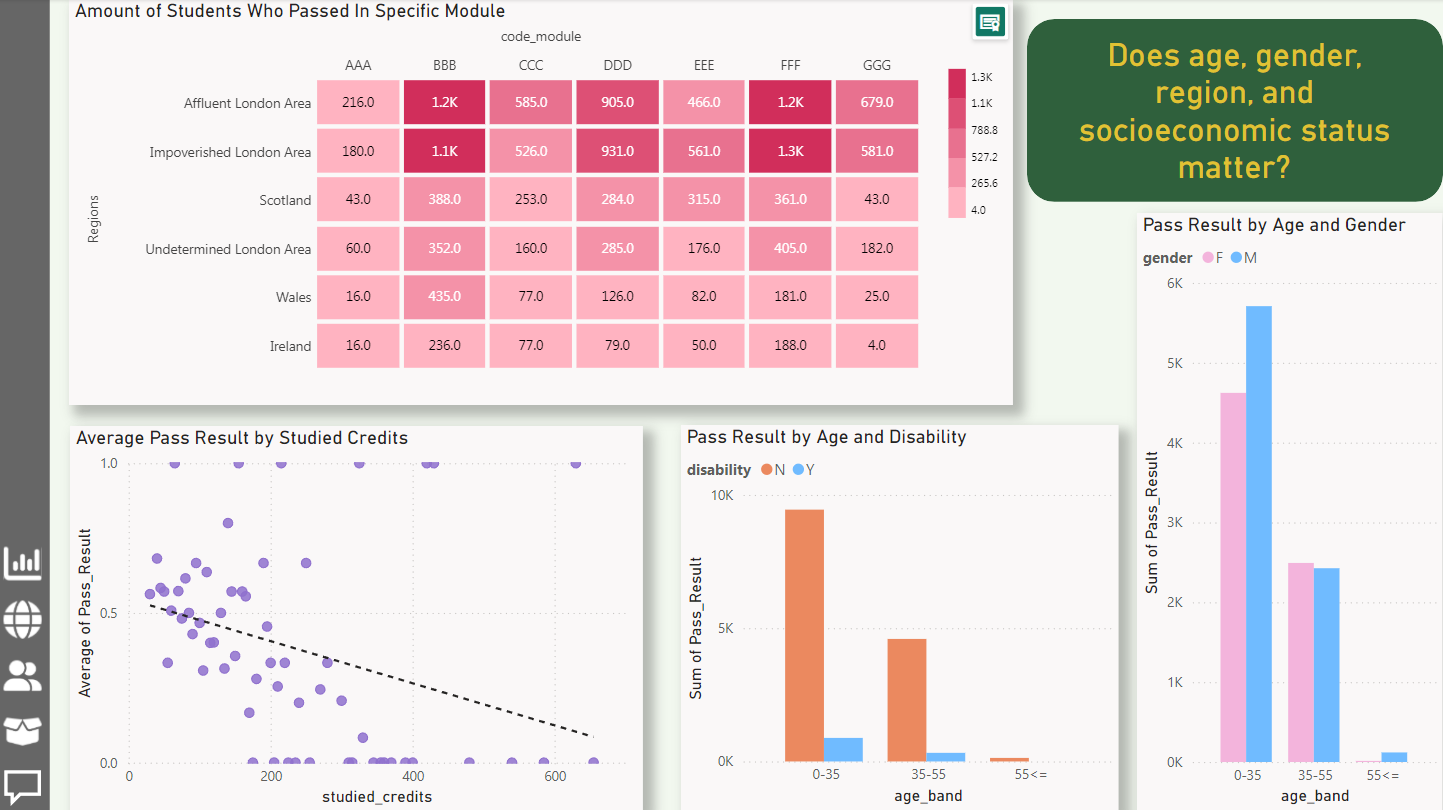
\includegraphics[width=0.45\textwidth]{photo/d2.PNG}\\
    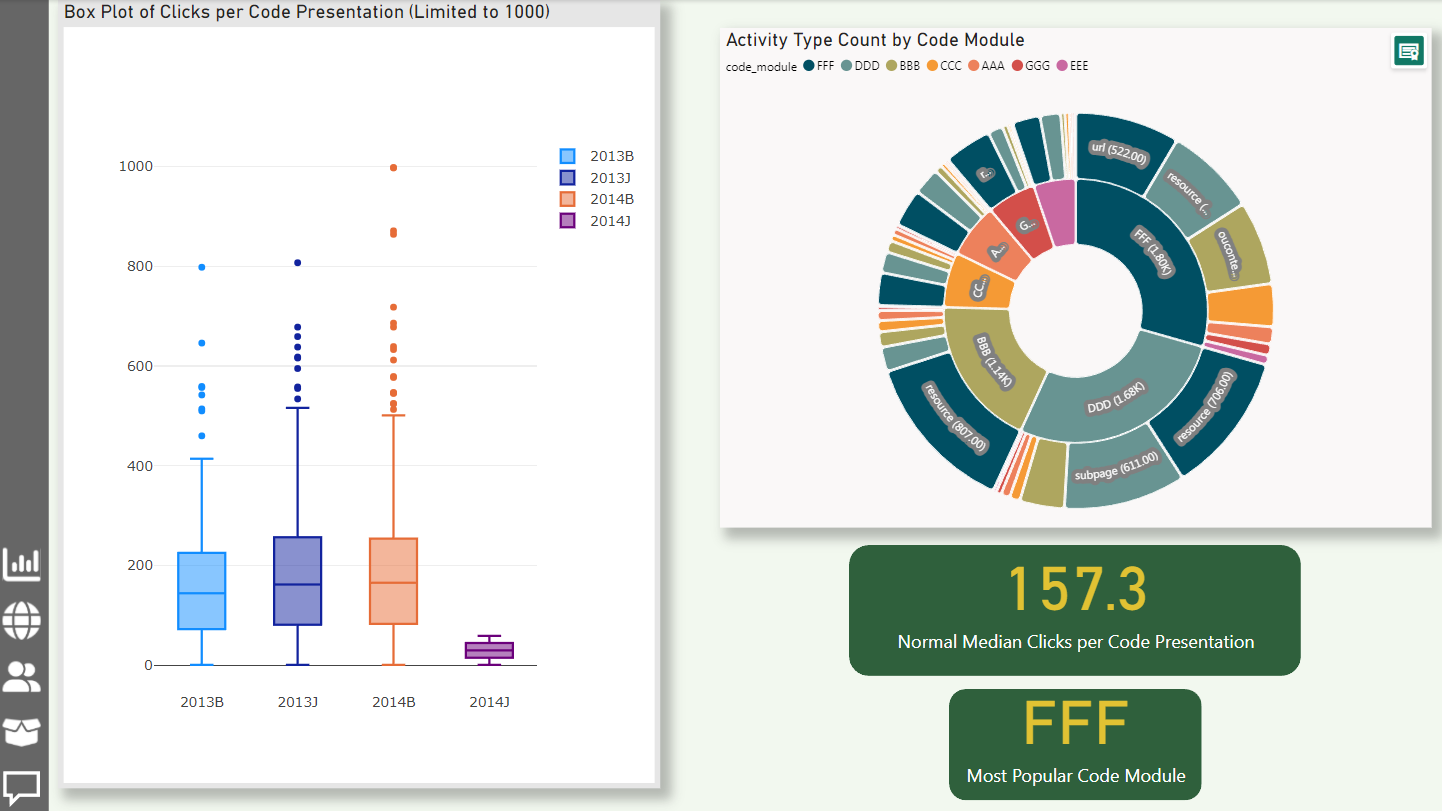
\includegraphics[width=0.45\textwidth]{photo/d3.PNG}
    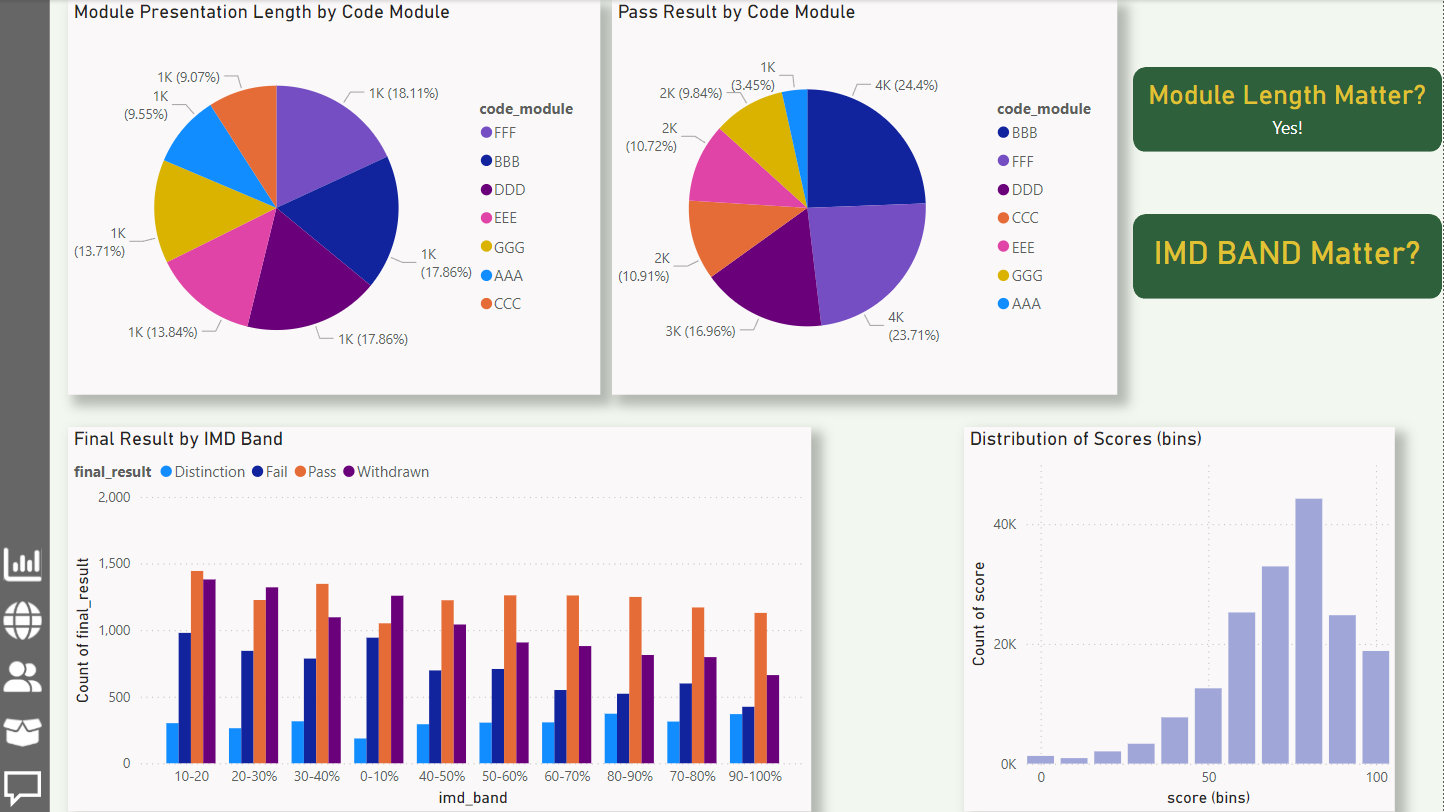
\includegraphics[width=0.45\textwidth]{photo/d4.PNG}
    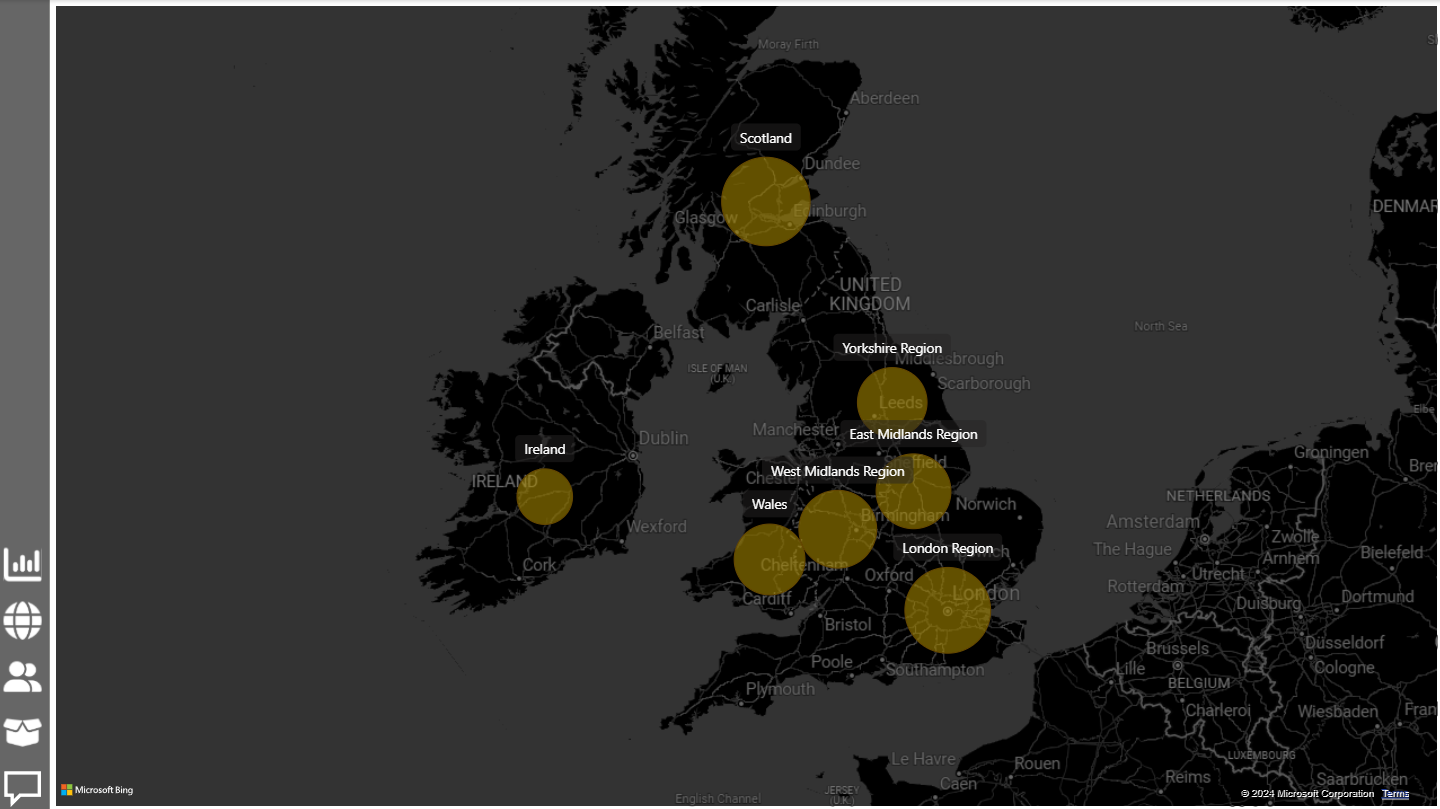
\includegraphics[width=0.45\textwidth]{photo/d5.PNG}
    \caption{Final Dashboards}
    \label{fig:multiple-images}
\end{figure}


\subsection*{Brief Dashboard Explanation (Top to bottom) (Figure~\ref{fig:multiple-images})}
\begin{itemize}
    \item \textbf{1: Overview of Engagement Metrics and Pass Rates} This figure provides an aggregated overview of student engagement and performance metrics across the dataset.
    
    \item \textbf{2: Impact of Demographics and Regional Factors} This figure examines the influence of demographic variables, including region, age, and disability status, on student performance.

    \item \textbf{3: Activity Types and Module Engagement} This figure explores student interaction levels across modules and activity types.

    \item \textbf{4: Module Presentation Length and Socioeconomic Factors} This figure delves into the relationship between module characteristics, student performance, and socioeconomic factors.

    \item \textbf{5: Student Map Pool} This is an interactive map that contains a clearer image of the regions the students are from (given that their region supports the map)

\end{itemize}

\subsection*{Overview of Engagement Metrics and Pass Rates}

The first set of visuals provides a high-level summary of student engagement and outcomes. Key metrics displayed include the average score (75.80), maximum total clicks (6,977), and overall pass rate (37.93%). These aggregate figures establish a baseline for deeper analysis, highlighting general trends within the dataset.

The scatter plot depicting the relationship between total clicks and scores reveals a positive correlation, indicating that students with higher Virtual Learning Environment (VLE) activity tend to achieve higher scores. However, the presence of outliers—students with high click counts but low scores—suggests that increased activity does not universally translate to better performance. This observation challenges the assumption that all engagement is productive and underscores the need to distinguish between meaningful interactions and aimless navigation.

The bar chart highlighting the most popular activity type, \textit{resource}, emphasizes its significance in driving student interaction. This insight prompts further exploration into why resource activities outperform other types such as \textit{subpage} and \textit{outcontent}, potentially informing strategies to enhance less engaging content.

The table displaying total pass rates by region reveals significant disparities. For example, students in Ireland exhibit the highest pass rates, while regions like Scotland and the Impoverished London Area have lower success rates. These findings raise important questions about the impact of socioeconomic and geographic factors on student outcomes, suggesting the need for targeted interventions to address regional disparities.

\subsection*{Impact of Demographics and Regional Factors}

The second set of visuals delves into the role of demographics—including region, age, and disability status—on student performance. The heatmap effectively illustrates the number of students passing specific modules across regions, with modules like \textit{FFF} and \textit{BBB} standing out in both Affluent and Impoverished London areas \cite{IMD2019}. This indicates that these modules are central to student success and may warrant further analysis to identify best practices that can be replicated elsewhere.

The scatter plot examining pass results by studied credits reveals a surprising negative trend: students with higher studied credits often have lower average pass results. This finding challenges the traditional assumption that taking more credits leads to better outcomes and may reflect issues such as student overextension or inadequate support for those with heavier workloads.

The bar chart comparing pass results by age group and disability status serves as a crucial tool for evaluating inclusivity and equity. The data show that students aged 0--35 consistently outperform older cohorts, and students without disabilities achieve higher pass rates than those with disabilities. These insights highlight the need for targeted support for older students and those with disabilities, such as tailored resources or additional academic counseling.

\subsection*{Activity Types and Module Engagement}

The third set of visuals examines student engagement concerning activity types and module participation. The box plot visualizing activity levels across different presentations (e.g., 2013B, 2014B) highlights variability in engagement over time. While most students engage at moderate levels, the presence of extreme outliers—particularly in the 2014B session—suggests that certain presentations or modules may drive unusually high engagement, warranting further investigation.

The sunburst chart showcasing the count of activity types by module identifies \textit{FFF} as the most popular module and \textit{resource} as the dominant activity type. This visualization underscores the importance of \textit{FFF} in shaping engagement trends and suggests that resource activities are particularly effective at engaging students. However, further evaluation of the quality and content of these resources is necessary to confirm this assumption.

\subsection*{Module Presentation and Socioeconomic Factors}

The fourth set of visuals explores the relationship between module length, pass results, and socioeconomic factors. The pie chart depicting the sum of module presentation lengths by code module indicates that modules like \textit{FFF} and \textit{BBB} account for a significant portion of student engagement. The corresponding pie chart for pass results mirrors this trend, reinforcing the link between module length and student success.

The bar chart of final results by Index of Multiple Deprivation (IMD) band provides a detailed examination of how socioeconomic status impacts student outcomes. Students from lower IMD bands—representing more deprived areas—are more likely to fail or withdraw, while those from higher bands achieve better results. This finding reinforces the assumption that socioeconomic disparities significantly influence educational success and underscores the need for policy interventions to address these gaps.

The histogram of scores, presented in bins, illustrates the distribution of student performance. The majority of students cluster around mid-range scores, with fewer achieving extremely high or low scores. This distribution meets our expectations for a diverse student population but also highlights the potential for targeted interventions to help more students achieve higher performance levels.

\begin{figure}[h]
    \centering
    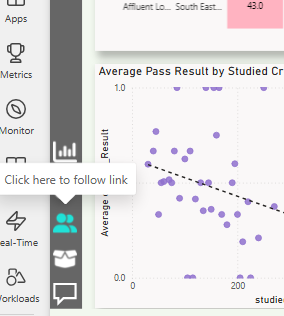
\includegraphics[width=\linewidth]{photo/buttonim.png}
    \caption{Example of button implementation for user navigation}
    \label{buttonim}
\end{figure}

\begin{figure}[h]
    \centering
    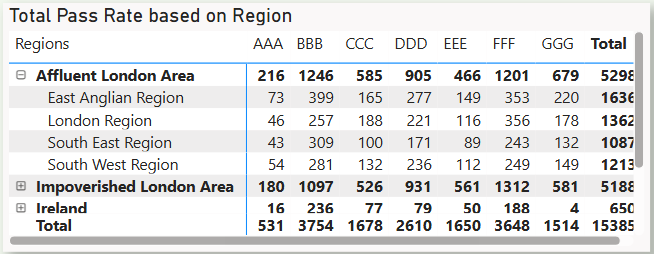
\includegraphics[width=\linewidth]{photo/hierarchy.PNG}
    \caption{Example of region hierarchy implementation for drilling up and down}
    \label{hierar}
\end{figure}

\begin{figure}[h]
    \centering
    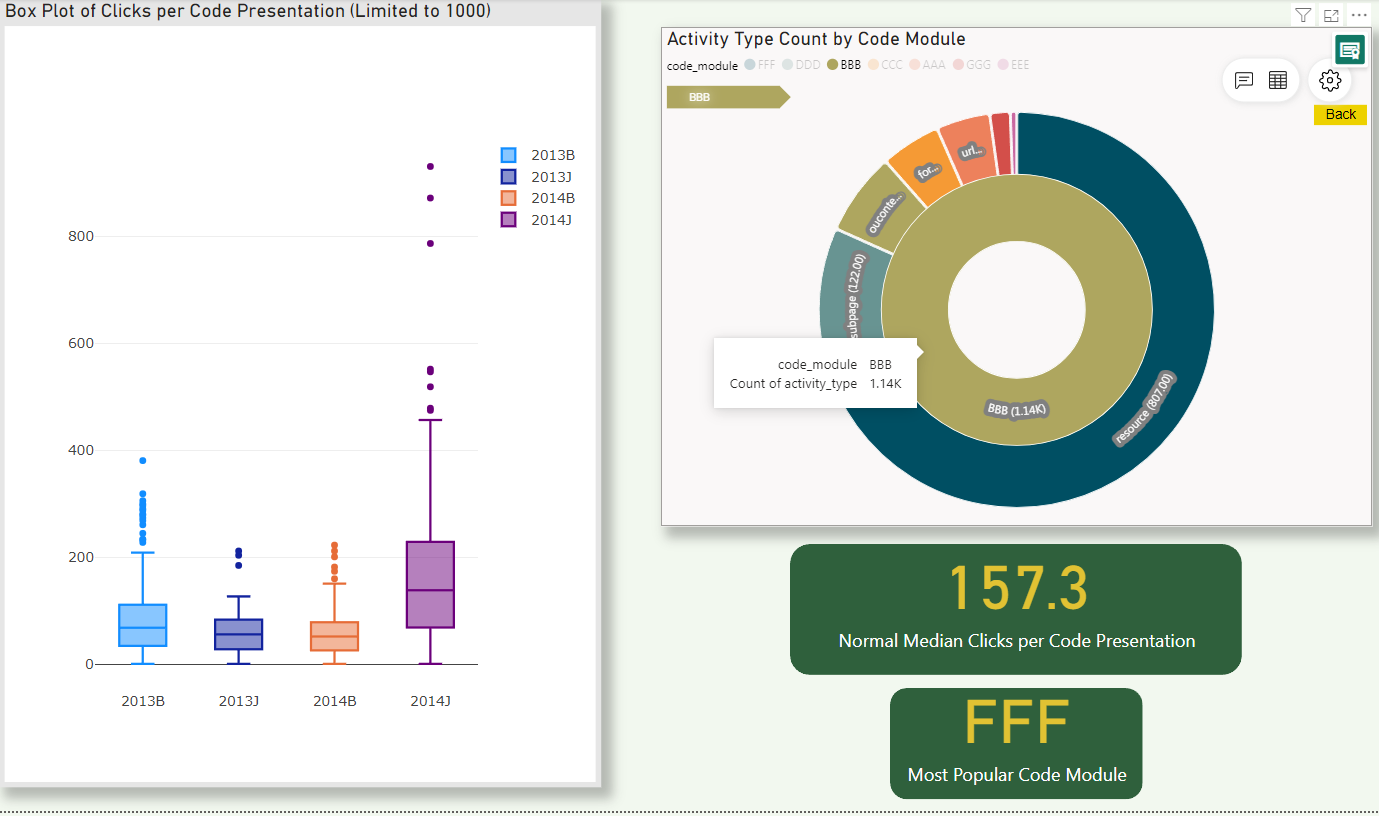
\includegraphics[width=\linewidth]{photo/changing.png}
    \caption{Dashboard changing once user interacts with visual (refer to third figure of the Final Dashoards images}
    \label{changin}
\end{figure}


\subsection*{Interactivity and User Experience}

An important aspect of the dashboard's design was enhancing interactivity to improve user experience. We ensured that the visuals were interactive, allowing users to effortlessly drill down or up to explore specific data visualizations based on their interests as demonstrated in Figure~\ref{changin}. Specifically, hierarchies were created within the regions column, enabling users to categorize data and focus on certain regions if desired as depicted in Figure~\ref{hierar}. This approach not only enhanced the performance of the visualizations by optimizing data loading and rendering but also significantly improved the user experience. Navigation buttons were also added on the bottom left to ensure that users can maneuver easily through each board as shown in Figure~\ref{buttonim}. Alongside this we made shapes with bold text to highlight key points or bring attention to specific details of the dashboard. By making the data more accessible and customizable, users can engage with the dashboard more effectively, leading to deeper insights and more informed decision-making.

\subsection*{Reflection on Assumptions}

Throughout the evaluation, we critically examine the assumptions underpinning our analysis. While trends such as the positive correlation between clicks and scores or the dominance of \textit{FFF} and \textit{resource} activities are supported by the data, the presence of outliers and counterintuitive findings—such as the negative correlation between studied credits and pass rates—prompt deeper reflection. These observations challenge simplistic narratives and shows the need for thorough, context-specific interpretations.

\subsection*{Evaluation Conclusion}

The dashboard effectively evaluates student engagement and performance through a diverse array of well-designed visuals. Each graph contributes to a comprehensive understanding of the dataset, highlighting key patterns and providing actionable insights. By incorporating interactive features and enhancing user experience, we have made the data more accessible and customizable, facilitating deeper exploration. Critically reflecting on assumptions and addressing anomalies, the evaluation aligns with our objectives and offers a thorough assessment of the results and their implications for improving online education.

\section{Deployment}

The deployment of the dashboard prioritizes user accessibility and scalability. Hosted on Power BI, the dashboard can be integrated into institutional systems—such as a university's learning management system—providing faculty and administrators with timely insights. The design ensures responsiveness to dynamic updates, including the incorporation of new student records or changes in course structures, by automating data refresh schedules within Power BI.

Scalability is addressed by optimizing the underlying data model to support large datasets without significant performance degradation, which is crucial given that one of our datasets, \texttt{studentVLE}, contains over 10 million rows. Additionally, the dashboard anticipates multi-user scenarios, accommodating concurrent access by various stakeholders while maintaining optimal performance.

In real-world applications, the dashboard serves as a tool to improve student outcomes. It enables early identification of at-risk students by visualizing patterns in engagement and performance metrics. For instance, modules with disproportionately low pass rates can prompt targeted interventions, such as implementing tailored teaching methods or providing additional resources. Demographic trends revealed through the visuals—such as those related to age and disability status—can inform policy decisions aimed at offering extra support to underrepresented groups.

\section{Conclusion}

The rapid shift toward online education has presented both opportunities and challenges in enhancing student engagement and performance. This study leveraged the Open University Learning Analytics Dataset (OULAD) to gain a comprehensive understanding of the factors influencing student success in virtual learning environments. Through meticulous data preparation, modeling, and visualization, we identified significant correlations between student demographics, engagement patterns, and academic outcomes.

Our analysis revealed that higher levels of interaction with VLE materials generally correlate with improved academic performance, underscoring the importance of fostering active engagement in online courses. However, the presence of outliers indicates that increased activity does not universally translate to better outcomes, suggesting that the quality of engagement is as crucial as the quantity. Furthermore, disparities in pass rates across different regions, age groups, and disability statuses highlight the impact of demographic and socioeconomic factors on student success, emphasizing the need for targeted support and inclusive educational strategies.

The deployment of an interactive dashboard using Power BI provides educators and administrators with a valuable tool for monitoring student engagement and identifying at-risk individuals or modules. This facilitates timely interventions and the implementation of personalized learning strategies aimed at improving retention and academic achievement.

In conclusion, this research demonstrates the efficacy of utilizing learning analytics to enhance online education. By analyzing the OULAD dataset and deploying actionable insights through data visualization, we contribute to the development of more effective, equitable, and personalized online learning environments. Future work could expand upon this study by incorporating real-time data analytics, exploring predictive modeling techniques for early identification of at-risk students, and extending the analysis to include additional variables such as student feedback and psychological factors.


% if have a single appendix:
%\appendix[Proof of the Zonklar Equations]
% or
%\appendix  % for no appendix heading
% do not use \section anymore after \appendix, only \section*
% is possibly needed

% use appendices with more than one appendix
% then use \section to start each appendix
% you must declare a \section before using any
% \subsection or using \label (\appendices by itself
% starts a section numbered zero.)
%

% ============================================
%\appendices
%\section{Proof of the First Zonklar Equation}
%Appendix one text goes here %\cite{Roberg2010}.

% you can choose not to have a title for an appendix
% if you want by leaving the argument blank
%\section{}
%Appendix two text goes here.


% use section* for acknowledgement
%\section*{Acknowledgment}


%The authors would like to thank D. Root for the loan of the SWAP. The SWAP that can ONLY be usefull in Boulder...


% Can use something like this to put references on a page
% by themselves when using endfloat and the captionsoff option.
\ifCLASSOPTIONcaptionsoff
  \newpage
\fi



% trigger a \newpage just before the given reference
% number - used to balance the columns on the last page
% adjust value as needed - may need to be readjusted if
% the document is modified later
%\IEEEtriggeratref{8}
% The "triggered" command can be changed if desired:
%\IEEEtriggercmd{\enlargethispage{-5in}}

% ====== REFERENCE SECTION

%\begin{thebibliography}{1}

% IEEEabrv,

%\bibliographystyle{IEEEtran}
%\bibliography{IEEEabrv,Bibliography}
%\end{thebibliography}
% biography section
% 
% If you have an EPS/PDF photo (graphicx package needed) extra braces are
% needed around the contents of the optional argument to biography to prevent
% the LaTeX parser from getting confused when it sees the complicated
% \includegraphics command within an optional argument. (You could create
% your own custom macro containing the \includegraphics command to make things
% simpler here.)
%\begin{biography}[{\includegraphics[width=1in,height=1.25in,clip,keepaspectratio]{mshell}}]{Michael Shell}
% or if you just want to reserve a space for a photo:


\bibliographystyle{plain}
\bibliography{references}
%% if you will not have a photo at all:
%\begin{IEEEbiographynophoto}{Ignacio Ramos}
%(S'12) received the B.S. degree in electrical engineering from the University of Illinois at Chicago in 2009, and is currently working toward the Ph.D. degree at the University of Colorado at Boulder. From 2009 to 2011, he was with the Power and Electronic Systems Department at Raytheon IDS, Sudbury, MA. His research interests include high-efficiency microwave power amplifiers, microwave DC/DC converters, radar systems, and wireless power transmission.
%\end{IEEEbiographynophoto}

%% insert where needed to balance the two columns on the last page with
%% biographies
%%\newpage

%\begin{IEEEbiographynophoto}{Jane Doe}
%Biography text here.
%\end{IEEEbiographynophoto}
% ==== SWITCH OFF the BIO for submission
% ==== SWITCH OFF the BIO for submission



% You can push biographies down or up by placing
% a \vfill before or after them. The appropriate
% use of \vfill depends on what kind of text is
% on the last page and whether or not the columns
% are being equalized.

\vfill

% Can be used to pull up biographies so that the bottom of the last one
% is flush with the other column.
%\enlargethispage{-5in}



% that's all folks

\end{document}


